\documentclass[aspectratio=169,11pt]{beamer}
\usepackage[utf8]{inputenc}
\usepackage[T1]{fontenc}
\usepackage[english]{babel}
\usepackage{amsmath,amssymb}
\usepackage{graphicx}
\usetheme{default}
\usecolortheme{seahorse}
\setbeamertemplate{navigation symbols}{}
\setbeamertemplate{footline}[frame number]
\setbeamerfont{frametitle}{size=\Large}
\setbeamerfont{title}{size=\LARGE}
\setbeamersize{text margin left=7mm,text margin right=7mm}

\definecolor{accent}{RGB}{55,76,118}
\setbeamercolor{structure}{fg=accent}
\setbeamercolor{alerted text}{fg=red!70!black}

\title{The Economics of Bicycles for the Mind}
\subtitle{Agrawal, Gans \& Goldfarb (2025)\\[0.4em]
NBER Working Paper 34034}
\author{}
\date{}

\begin{document}

% 1 ------------------------------------------------------------------
\begin{frame}[plain]
  \titlepage
  \vspace{-1.1em}
  \begin{center}
    \small\url{https://github.com/carlosgomezp28/ai-02-agrawal}

    \vfill
    \footnotesize Repository 2 --- Artificial Intelligence and Economic Modeling
  \end{center}
\end{frame}

% 2 ------------------------------------------------------------------
\begin{frame}{The Paper: Cognitive Tools and Human Capabilities}
  \textbf{Question.} How do cognitive tools change productivity and the value
  of different human capabilities?

  \smallskip
  \begin{columns}[T,onlytextwidth]
    \column{0.32\textwidth}
      \textbf{Implementation skill $s$}
      \begin{itemize}
        \item Converts effort into successful implementation
        \item Tools substitute for it
      \end{itemize}

    \column{0.32\textwidth}
      \textbf{Opportunity judgment $\rho$}
      \begin{itemize}
        \item Recognizes further improvements
        \item Complements tools
      \end{itemize}

    \column{0.32\textwidth}
      \textbf{Payoff judgment $\eta$}
      \begin{itemize}
        \item Turns success into value
        \item Complementarity is conditional
      \end{itemize}
  \end{columns}

  \vspace{-0.2em}
  \begin{block}{Agent's problem}
    \vspace{-0.8em}
    \[
      M(e;\theta)=p(se;\theta)\eta\Delta-c(e;\theta),\qquad
      e^*(\theta)\in\arg\max_{e\geq0}M(e;\theta)
    \]
    \vspace{-1.0em}
    \[
      p_x(se;\theta)s\eta\Delta=c_e(e;\theta).
    \]
  \end{block}
  \vspace{-0.3em}
  \centering\emph{AI improves implementation technology, but the worker
  optimally changes effort in response.}
\end{frame}

% 3 ------------------------------------------------------------------
\begin{frame}{Main Results: Propositions 1--3}
  \small
  \begin{columns}[T,onlytextwidth]
    \column{0.29\textwidth}
      \begin{block}{Proposition 1}
        \[
          \begin{gathered}
            e^*(1)<e^*(0),\\[-0.2em]
            V_0(1)>V_0(0).
          \end{gathered}
        \]
        Less implementation effort,\\ greater total value.
      \end{block}

    \column{0.37\textwidth}
      \begin{block}{Proposition 2}
        \begin{itemize}
          \setlength\itemsep{0.15em}
          \item Opportunity judgment: complement
          \item Implementation skill: substitute if $p_{s\theta}<0$
          \item Payoff judgment: conditional complement
        \end{itemize}
        \vspace{-0.25em}
        \[
          \begin{aligned}
          \frac{dD}{d\eta}=\Gamma\Delta\bigl[&p(se^*(1);1)\\[-0.15em]
                                               &-p(se^*(0);0)\bigr].
          \end{aligned}
        \]
      \end{block}

    \column{0.30\textwidth}
      \begin{block}{Proposition 3}
        \[
          e(\theta)=\frac{\eta^2s}{4}-\frac{\theta}{s},
        \]
        \vspace{-0.65em}
        \textbf{Interiority:} $\eta^2s^2>4\theta$.
        \vspace{-0.35em}
        \[
          V(\theta)=G\left[\frac{\eta^2s}{4}+\frac{\theta}{s}\right].
        \]
      \end{block}
  \end{columns}

  \vspace{-0.55em}
  \begin{alertblock}{Condition (30): inequality initially falls}
    \vspace{-0.45em}
    \[
      \frac{E[G^2]}{(E[G])^2}<\bar{s}\,E[1/s].
    \]
  \end{alertblock}
\end{frame}

% 4 ------------------------------------------------------------------
\begin{frame}{What I Did}
  \begin{enumerate}
    \item Reconstructed the effort FOC and Proposition 2 envelope-theorem argument.

    \item Derived Proposition 3's variance from first principles:
      \[
        \operatorname{Var}(V(\theta))
        =A+a_0\theta+\theta^2\operatorname{Var}(G/s),
        \qquad
        \frac{d\operatorname{Var}(V(\theta))}{d\theta}
        =a_0+2\theta\operatorname{Var}(G/s).
      \]

    \item Separated total-value inequality from inequality in individual AI benefits:
      \[
        B_i(\theta)=V_i(\theta)-V_i(0)=\theta\frac{G_i}{s_i},
        \qquad
        \operatorname{Var}(B(\theta))=\theta^2\operatorname{Var}(G/s).
      \]

    \item Audited the assumptions behind the claimed U-shape.
  \end{enumerate}

  \begin{alertblock}{Takeaway}
    Unequal AI benefits can increase even while total outcome inequality initially falls.
  \end{alertblock}
\end{frame}

% 5 ------------------------------------------------------------------
\begin{frame}{Where I Did Not Believe AI}
  \small
  \begin{columns}[T,onlytextwidth]
    \column{0.72\textwidth}
      \textbf{Initial LLM claim:} ``Variance is globally U-shaped in $\theta$.''

      \smallskip
      \textbf{My check}
      \[
        e(\theta)=\frac{\eta^2s}{4}-\frac{\theta}{s}
        \qquad\text{requires}\qquad \eta^2s^2>4\theta.
      \]
      Therefore the interior formula cannot automatically be extended to all
      $\theta\geq0$.

    \column{0.24\textwidth}
      \centering
      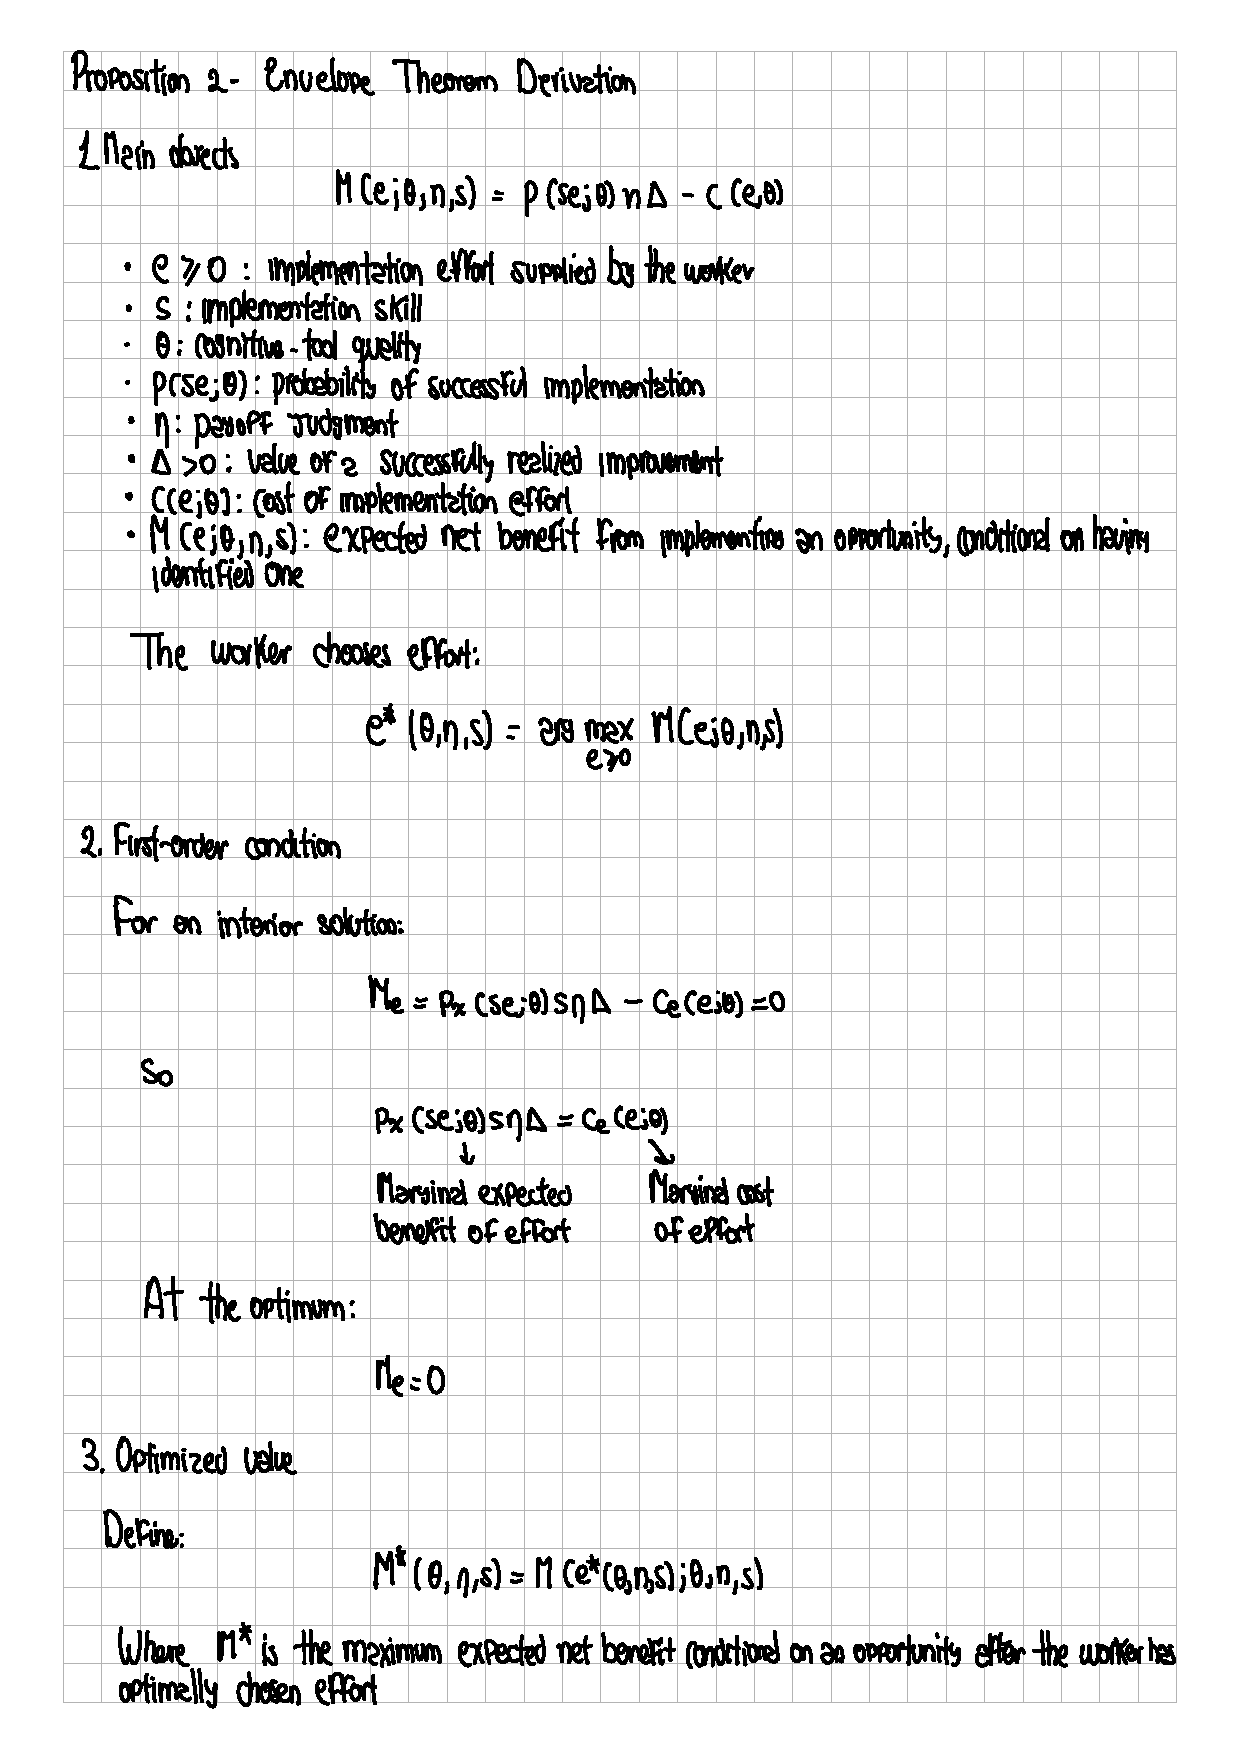
\includegraphics[page=1,width=\linewidth,height=0.23\textheight,keepaspectratio]
        {hand/prop-2-envelope-theorem.pdf}

      \scriptsize Handwritten envelope-theorem check
  \end{columns}

  \vspace{-0.4em}
  \[
    \frac{d^2\operatorname{Var}(V(\theta))}{d\theta^2}
    =2\operatorname{Var}(G/s)\geq0.
  \]
  \vspace{-0.75em}
  \begin{itemize}
    \setlength\itemsep{0.1em}
    \item Convex on the common interior domain.
    \item Condition (30) makes the initial slope negative.
    \item A U-shape additionally requires $\theta^*$ inside that domain.
  \end{itemize}

  \vspace{-0.35em}
  \begin{alertblock}{Verdict: referee concern, not a confirmed paper error}
    Eq.~(32)'s positive slope at $\theta=1$ is not implied by condition (30) alone.
  \end{alertblock}

  \vspace{-0.4em}
  \scriptsize The suspected coefficient-of-variation typo was retracted because
  PDF extraction may have omitted a square root.
\end{frame}

\end{document}
